\documentclass[12pt]{article}

% PACKAGES
\usepackage[a4paper,bindingoffset=0in,
            left=1in,right=1in,top=1in,bottom=1.5in,
            footskip=.5in]{geometry}
\usepackage{lastpage}
\usepackage[ddmmyyyy]{datetime}
\usepackage{amsmath}              % need for subequations
\usepackage{graphicx}             % need for figures
\usepackage{verbatim}             % useful for program listings
\usepackage{color}                % use if color is used in text
\usepackage{subfigure}            % use for side-by-side figures
\usepackage{hyperref}             % use for hypertext links, including those to external documents and URLs
\usepackage{fancyhdr}             % for image in header
\usepackage[table,xcdraw]{xcolor} % for color in cell
\usepackage{float}
\usepackage{tabularx}
\restylefloat{table}

\setlength{\parindent}{0pt}
\hypersetup{
    colorlinks=false,
    pdfborder={0 0 0},
}

%%%%%%%%%%%%%%%%%%%%%%%%%%%%%%%%%%%%%%%%%%%%%%%%%%%%%%%%%%%%%%%%%%%%%%%%%%%%%%%%%%%%%%%%%%%%%%%%%%%%%%%%%%

% HEADER and FOOTER
\pagestyle{fancy}{
  \lhead{
\includegraphics[width=4.5cm]{Images/Logos/logoUnimi}}
  \rhead{
\includegraphics[width=5cm]{Images/Logos/logoPong}}
  \lfoot{Last updated: \today}
  \cfoot{ }
  \rfoot{Page \thepage\ of \pageref{LastPage}}
}

\begin{document}

% logoTeam
\begin{center}
  \begin{figure}[H]
  \centering
  \vspace*{5\baselineskip}
  
\includegraphics[width=10cm]{Images/Logos/logoTeam}
  \end{figure}

  \vspace{50pt}
  {\huge \textbf{Sophie's Flying Castle}} \\
  {\large \textbf{ \textit{PONG - Game and Level Design}}}
\end{center}

\vspace{20pt}
\begin{table}[H]
  \centering
  \begin{tabular}{lcr}
    \textbf{Francesco Periti}	& \underline{\href{mailto:francesco.periti@studenti.unimi.it}{francesco.periti@studenti.unimi.it}}	& 930650 \\
    \textbf{Francesco Principe}	& \underline{\href{mailto:francesco.principe@studenti.unimi.it}{francesco.principe@studenti.unimi.it}}	& 937622 \\
    \textbf{Davide Valentini}	& \underline{\href{mailto:davide.valentini1@studenti.unimi.it}{davide.valentini1@studenti.unimi.it}}	& 939054 \\
    \textbf{Elena Coperchini}	& \underline{\href{mailto:elena.coperchini@gmail.com}{elena.coperchini@gmail.com}}			& \\
  \end{tabular}
\end{table}


  \vspace{10pt}
% TABELLA 1
\begin{table}[H]
  \centering
  \begin{tabular}{|l|l|}
    \hline
    \cellcolor{lightgray}\textbf{Purpose} &  Define rules for files and directories \\\hline
    \cellcolor{lightgray}\textbf{Creation date} & 02/11/2018 \\\hline
    \cellcolor{lightgray}\textbf{Current owner} & Francesco Periti \\\hline
%    \cellcolor{lightgray}\textbf{Last update} & \today \\\hline
  \end{tabular}
\end{table}

\clearpage

\section*{Revision History}
% TABELLA 2
\begin{table}[H]
\centering
  \begin{tabularx}{\textwidth}{|l|l|X|}
\hline
\cellcolor{lightgray}\textbf{Who} & \cellcolor{lightgray}\textbf{When} & \cellcolor{lightgray}\textbf{What} \\ \hline
Francesco Periti & 02/11/2018 & Created this document \\ \hline
Francesco Periti & 03/11/2018 & Added some conventions to directory structure \\ \hline
Davide Valentini & 03/11/2018 & Added e-mail references \\ \hline
Francesco Principe & 04/11/2018 & Added some conventions to file naming \\ \hline
Davide Valentini & 04/11/2018 & Added software list \\ \hline
Francesco Principe & 05/11/2018 & Global revision \\ \hline
Davide Valentini & 06/11/2018 & Added file access rules \\ \hline
Francesco Periti & 06/11/2018 & Added repository structure rules \\ \hline
Davide Valentini & 07/11/2018 & Added owners and editors rules \\ \hline
Francesco Periti & 08/11/2018 & Global revision \\ \hline
Francesco Periti & 18/11/2018 & Added game title \\ \hline
\end{tabularx}
\end{table}

\clearpage

\section{Software List}

\subsection{Asset Editing Software}
\textbf{Photoshop CC 2018} for 2D bitmap images.
\textbf{Inkscape 0.92+} for SVG images.

\subsection{Development Software}
\textbf{Neverwinter Nights Toolset} for level prototype.

\subsection{Organization Software}
\textbf{TexMaker with MiKTeX 2.9} for editing tex files.

\textbf{git} for files versioning.

\subsection{Environments}
\textbf{Windows 10}

\section{Data Types and Format}

\subsection{Date format}
DD/MM/YYYY

\subsection{Text}
\textbf{Formats}: tex (LaTeX).

%Use 4-spaces \textbf{tabs} for indentations.

Use \textbf{double return} to break paragraphs.

Use '\textbf{H}' to place floats (e.g. images and tables) in their correct position. Example: \textit{\textbackslash{}begin\{figure\}[H]}

Every LaTeX files has 100\% compatibility with any other LaTeX file.

\subsection{Images}
\textbf{Formats for assets}: tif/tiff, svg.

\textbf{Formats for documentation}: png.

\textbf{Formats for reference images}: tif/tiff, png, svg, jpeg, jpg, bmp, gif.

Size (W x H) and editing software are defined by the following rules:
\begin{itemize}
	\item \textbf{\path{./Documents/Images/Characters}}: 250px x 350px, Photoshop
	\item \textbf{\path{./Documents/Images/SVG/Exported/Circumplexes}}: 1321px x 895px, exported from \path{./Documents/Images/SVG/circumplexes.svg}
	\item \textbf{\path{./Documents/Images/SVG/Exported/Evolutions}}: 1321px x 895px, exported from \path{./Documents/Images/SVG/evolutions.svg}
	\item \textbf{\path{./Documents/Images/SVG}}: Inkscape
\end{itemize}

\subsection{Audio}
%Audacity

\textbf{Formats for assets}: flac.

\textbf{Formats for reference audios}: mp3.

Software to be defined.

Contact one of the project owners:
\begin{itemize}
	\item francesco.periti@studenti.unimi.it
	\item francesco.principe@studenti.unimi.it
	\item davide.valentini1@studenti.unimi.it
\end{itemize}

Bit rate: 96kbps+

Sampling rate: 44.1-48KHz

Channel: stereo (if available)

\subsection{Video}
\textbf{Formats for assets}: mkv, avi, mp4.

\textbf{Formats for reference videos}: mkv, avi, mp4, flv.

Software to be defined.

Contact one of the project owners:
\begin{itemize}
	\item francesco.periti@studenti.unimi.it
	\item francesco.principe@studenti.unimi.it
	\item davide.valentini1@studenti.unimi.it
\end{itemize}

Resolution: 1920x1080px (preferred), 2K, 4K, 1280x720px

FPS: 24+

\subsection{3D Models}
\textbf{Formats}: to be defined.

Software to be defined.

Contact one of the project owners:
\begin{itemize}
	\item francesco.periti@studenti.unimi.it
	\item francesco.principe@studenti.unimi.it
	\item davide.valentini1@studenti.unimi.it
\end{itemize}

Maximum number of triangles: to be defined.

Scale: to be defined.

\section{Data Storage and Access}
Project data are stored on a private git repository:\\
	\textit{git@pong.di.unimi.it:GLD/18/teamdellelande}

The repository structure follows the good pratices of GitFlow.

The history graph can become very complex; in order to avoid that, you have to work with two type of branches:
\begin{itemize}
	\item branches with infinite lifetime
	\item branches with finite lifetime
\end{itemize}

\subsection{Branches with infinite lifetime}
They are the main branches of the project. There are two different infinite lifetime branches:
\begin{itemize}
\item \textbf{master}: this branch contains the last project review locked down by the project responsible.

  Only with the last version on master it can be done the \textit{level design to art handoff}.

  You have not to do any commit/merge in this branch unless the project responsibles agree that the current version can be \textit{locked-down}.

\item \textbf{develop}: This branch is the development branch. Each one has to work and make his own changes to it.

  When you think you had made a good change, you have to do a commit inside here so others can use it.
  If the project responsibles agree that the current version can be \textit{locked-down} the develop will be merged on the \textit{master} branch and a TAG version will be binded to that commit.
\end{itemize}

\subsection{Branches with finite lifetime}
You work on them just for a certain period and then you have to delete them.

You have to work on one branch at a time.

When you want to add a new content you have not to work on \textit{develop} branch.

You have to create a temporary branch where you can work and only when you have finished it you have to merge your branch with the \textit{develop} branch.

%You will never use more this branch so delete it. When you will want to add new content you have to make a new branch e so on.

\subsection*{Synthesis}
When you work on a new content, you have to work on a temporary branch and when you have finished you have to merge your commits with the \textit{develop} branch.\\
\textit{New content? New branch}.\\
\textit{Work completed? Merge with develop}.\\
%And so on.

\subsection*{Revision history}
Whenever you make a commit or a merge with the \textit{develop} branch, you must add a comment about your work in the revision history file: \path{./Documents/revisionHistory.tex}.

\subsection{Data access and permissions}
The following table indicates \textit{owners} and \textit{editors} for files.

Only the \textit{editors} are allowed to add and edit files.

Only the \textit{owners} are allowed to enable new \textit{editors}, edit the folder and add subfolders. The \textit{owners} are not allowed to edit files (unless they are also \textit{editors}).

To avoid merging non-text files, nobody has to add/edit non-text files in any directory, unless he is the owner of the directory and that is a subdirectory of the Images directory.

Everybody can read all the files.

Rules are sorted by priority: first rule has the highest priority and overwrites the others.

\begin{table}[H]
\centering
  \begin{tabularx}{\textwidth}{|X|p{3.5cm}|X|}
\hline
\cellcolor{lightgray}\textbf{Files} & \cellcolor{lightgray}\textbf{Owner} & \cellcolor{lightgray}\textbf{Editors} \\ \hline
\path{./Documents/Images/Characters/*} & Francesco Principe & Francesco Principe \\ \hline
\path{./Documents/Images/Logos/*} & Francesco Periti & Francesco Periti \\ \hline
\path{./Documents/Images/SVG/*} & Davide Valentini & Davide Valentini \\ \hline
\path{./Documents/Images/*} & Francesco Periti & Francesco Principe, Francesco Periti, Davide Valentini \\ \hline
\path{./Documents/*.tex} & Francesco Principe & Every member of the Wastelands Team \\ \hline
\path{./*} & Francesco Principe, Francesco Periti, Davide Valentini & Francesco Principe, Francesco Periti, Davide Valentini \\ \hline
\end{tabularx}
\end{table}

\subsection{Backup}
There are daily backups on three different machines in three different locations.

Responsibles:
\begin{itemize}
	\item \textbf{Francesco Periti} for Piacenza
	\item \textbf{Francesco Principe} for Parma
	\item \textbf{Davide Valentini} for Milan
\end{itemize}

\section{Directory Structure}
\begin{center}
  \begin{figure}[H]
  \centering
  %\vspace*{5\baselineskip}
  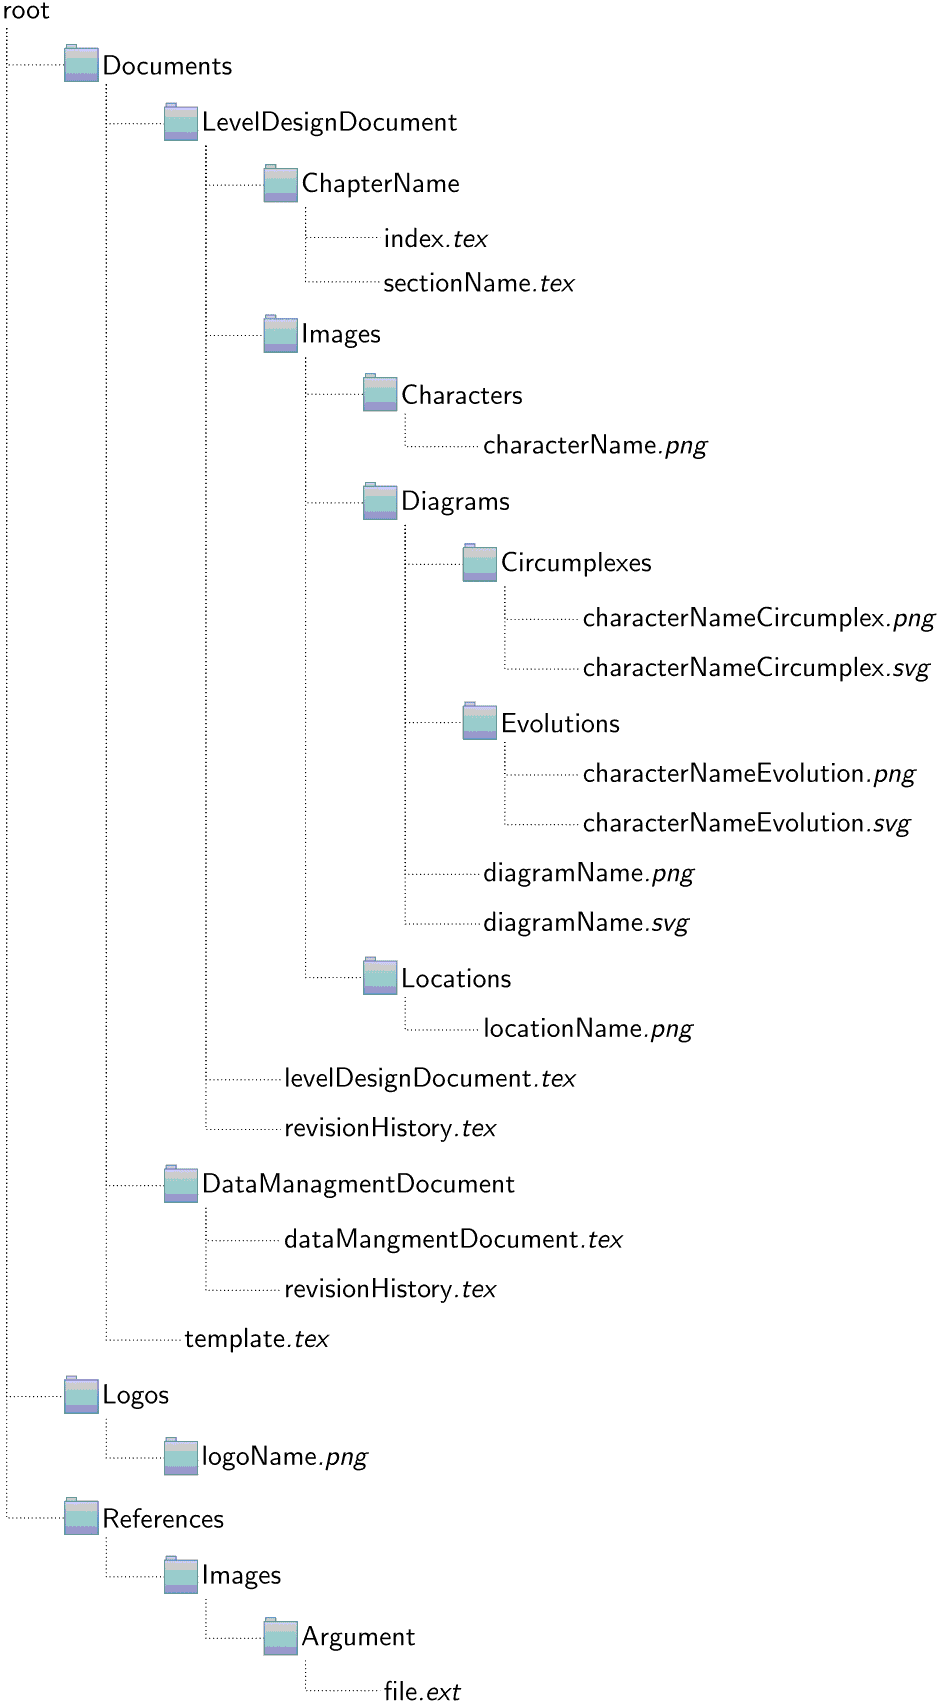
\includegraphics[width=10cm]{DataMangmentDocument/directories}
  \end{figure}
\end{center}
\begin{itemize}
\item \textbf{\path{./Documents}}: contains a directory for each document and a template that has to be used for eventual new documents.
  \begin{itemize}
    \item \textbf{\path{./DataManagmentDocument}}: contains the data managment document, where you find all technical features and rules to work on the project, and the relative revision history.

    \item \textbf{\path{./LevelDesignDocument}}: contains the level design document, where you find everything about the game and level, the relative revision history, a directory containing images for the whole project and a directory for each chapter. Each chapter subfolder has its own section files and a "index.tex" file.
    \begin{itemize}
    \item \textbf{\path{./Images}}: contains every image for the level design documentation. There are some subfolders:
    \begin{itemize}
      \item \textbf{\path{/Characters}}: contains one portrait for each character.
      \item \textbf{\path{/Diagrams}}: contains all diagrams file used in the level design document. If the diagram is a circumplex or an evolution it has to be placed in the relative subfolder.
        \item \textbf{\path{/Locations}}: contains one picture for each location.
        \item \textbf{\path{/Maps}}: contains all the maps used in the level design document.
    \end{itemize}
\end{itemize}
\end{itemize}
    \item \textbf{\path{./Logos}}: contains all the logos (\textit{.png} file) used in the level design document.

    \item \textbf{\path{./ReferenceImages}}: this directory contains all the LaTeX files about the story.

\end{itemize}

\section{File Naming Convention}
\subsection{General conventions}
During the project development has always to be respected the following generic conventions:
\begin{itemize}
  \item The name of each file has to begin with a lowercase character. Each time you want to separate two words within a file name, you have not to add a space between them but you have to make the first character of the second word uppercase: \textit{fileNameExample.ext}
  \item The name of each folder has to begin with an uppercase character. Each time you want to separate two words within a directory name, you have not to add a space between them but you have to make the first character of the second word uppercase: \textit{FolderNameExample}
   \item Files named \textit{index.tex} are used as containers, they connect all the other files inside the current directory. Each chapter directory has to contain one.
\end{itemize}
\subsection{Specific conventions}
File naming has to respect some conventions in according to the current work directory:
\begin{itemize}
  \item LevelDesignDocument:\\
  Each directory inside this is bound with a chapter. So, each chapter has its own directory named with own name. If you want add a chapter you have to add also the relative directory.
  \item Inside a chapter directory, each file has to have as a name the name of a section of the chapter.\\
  If you want add a section you have to add also the relative file.
  \item Images\/Characters:\\
  The name of each file inside here has to be the concatenation of three strings:
  \begin{enumerate}
    \item the name of character represented. If there are represented more characters you have to link their name with "+" (e.g. Howl+Calcifer).
    \item the current date (e.g. 2018-1-1)
    \item the character "\#" followed by the current number of file with this name plus one.
  \end{enumerate}
  If there are five image about Sophie and Howl and all of them are added today, your next image about Sophie and Howl (if you add it today) is: \textit{Sophie+Howl2018-1-1\#6}
  \item Images\/Locations:
  The name of each file inside here has to be the concatenation of three strings:
  \begin{enumerate}
    \item the name of location represented. If there are represented more location you have to link their name with "+" (e.g. Wastelands+SouthernDesert).
    \item the current date (e.g. 2018-1-1)
    \item the character "\#" followed by the current number of file with this name plus one.
  \end{enumerate}
  If there are five image about Southern Desert and all of them are added today, your next image about it (if you add it today) is: \textit{SouthernDesert2018-1-1\#6}
  \item Images\/Map:
  The name of each image inside here has to be the concatenation of three strings:
  \begin{enumerate}
    \item the name of level represented. If there are represented more level you have to link their name with "+".
    \item the current date
    \item the character "\#" followed by the current number of file with this name plus one.
  \end{enumerate}
  \item Images\/Logs:
  The name of each image inside here has to be the concatenation of two strings:
  \begin{enumerate}
    \item "logo"
    \item the argument of the logo.
  \end{enumerate}
  If you want add a logo about a program named "RPG Maker" for example, you have to name this logo \textit{logoRpgMaker}.
  \item Images\/SVG: \\Each file with extension \textit{.svg} has to have the corrispective file (with the corrispective name) in the exported directory with the extension \textit{.png}.
  \item Images\/References\/Illustrations:\\
  he name of each image inside here has to be the concatenation of three strings:
  \item name,"+",surname of illustrator (e.g. elena+coperchini)
  \item name of subject illustrated. An example may be a name character if the subject is the character.
  \item date
  %\item the character "\#" followed by the current number of file with this name plus one.
  %E.g. elena+coperchiniBelzel2018-1-1#0

\end{itemize}
\end{document}
